\documentclass[twocolumns, a4paper,10pt,fleqn]{extarticle}
\usepackage[english]{babel} 
\usepackage[latin1]{inputenc} 
\usepackage{times}			% Default times font style
\usepackage[T1]{fontenc} 	% Font encoding
\usepackage{amsmath} 		% Math package
\usepackage{mathtools} 		% Adds the declare paired 
							% delimeter command to make costom \abs and \norm
\usepackage{breqn}		 	% Adds dmath environment for automated brakeline
\usepackage{xfrac}			% Adds slanted fractions (sfrac)
\usepackage{cancel}			% Adds the cancel command, a slash through the symbol(s)
\usepackage{tabularx}		% Adds adjustable width on tabulars
\usepackage{cuted}			% Adds the strip command, pagewidth text in a twocolumn
							% environment.  
\usepackage{hyperref}
\usepackage[a4paper, margin=0.6in]{geometry}


% Alghorithm packages:
\usepackage{algorithm}
\usepackage[noend]{algpseudocode}

% Start custom \abs \norm 
\DeclarePairedDelimiter\abs{\lvert}{\rvert}%
\DeclarePairedDelimiter\norm{\lVert}{\rVert}%
% Swap the definition of \abs* and \norm*, so that \abs
% and \norm resizes the size of the brackets, and the 
% starred version does not.
\makeatletter
\let\oldabs\abs
\def\abs{\@ifstar{\oldabs}{\oldabs*}}
%
\let\oldnorm\norm
\def\norm{\@ifstar{\oldnorm}{\oldnorm*}}
\makeatother
% End custom \abs \norm 

\usepackage{titlesec}
\titleformat{\section}[block]{\bfseries\filcenter}{\thesection}{1em}{\uppercase}
\titleformat{\subsection}[hang]{\bfseries\filcenter}{\thesubsection}{1em}{}
\titleformat{\subsubsection}[hang]{\bfseries\filcenter}{\thesubsubsection}{1em}{}

% TODO: Put comments on this section.
\newcommand{\eq}[1]{{\small\begin{align*}#1\end{align*}}}
\newcommand{\equ}[1]{{\small\begin{align}#1\end{align}}}
\newcommand{\mat}[1]{\begin{matrix}#1\end{matrix}}
\newcommand{\pmat}[1]{\begin{pmatrix}#1\end{pmatrix}}
\newcommand{\bmat}[1]{\begin{bmatrix}#1\end{bmatrix}}
\newcommand{\vmat}[1]{\begin{vmatrix}#1\end{vmatrix}}
\newcommand{\ket}[1]{|#1\rangle}
\newcommand{\bra}[1]{\langle#1|}
\newcommand\numberthis{\addtocounter{equation}{1}\tag{\theequation}}
\newcommand{\Int}[4]{\int_{#1}^{#2} \! \mathrm{d}#3 \, #4}
\renewcommand\vec[1]{\boldsymbol{\mathbf{#1}}}
\newcommand{\OP}[1]{\mathbf{\widehat{#1}}}
\newcommand{\op}[1]{\hat{#1}}
\newcommand{\unit}[1]{\mathbf{\hat{#1}}}
\renewcommand{\thesection}{\Roman{section}}
\renewcommand{\thesubsection}{\Alph{subsection}.}
\renewcommand{\thesubsubsection}{\roman{subsubsection}.}
\newcommand{\Var}[1]{\mathrm{Var}(#1)}

\title{}

\begin{document}

\twocolumn[{%
 \centering
 {\bfseries\large Variational Monte-Carlo Simulations of Atomic Systems}
 \\[1em]
 \normalsize Daniel Marelius Bj\o rnstad and Alexander Fleischer
 \\
 \small\url{https://github.com/lastis/FYS4411}
  \begin{abstract}
    This project aims to find good approximations to the ground state energies
    of the atoms Helium, Beryllium and Neon, and the di-molecules $H_2$ and $Be_2$
    This was achieved by implementing the Variational Monte Carlo method of
    Metropolis-Hastings.
    The trial wave function of the 
    The variational parameters of the method was optimized using
    Nonlinear Conjugate Gradient method.
    To evaluate the results of the numerical methods, we investigated the possibility
    of finding a closed-form solution of the ground-state energy 
    using the Variational Principle.
    We also applied the statistical method of blocking to evaluate
    the variance in our results.
  \end{abstract}
 \\[3em] % some more space after the title part
}]

\section{Introduction} 
The aim of the project is to estimate the ground state energies of the
atoms (Hydrogen, Helium, Beryllium and Neon) and some simple molecules ($H_2$ and $Be_2$).

In the method and theory section (II), 
we first discuss some elements of the quantum mechanical system 
of the atoms and molecules.
We then outline the methods used to produce the results --
the Monte Carlo method with the Metropolis test, how the trial wave functions
of the variational principle may be found, and what kind of functions we have used.
The main part of the project focuses on the Hydrogen-like wave functions,
but we also use wave functions of Gaussian-type orbitals (GTOs).
We discuss the Slater determinant part and the addition of a
correlation part called the Pad\'e-Jastrow factor.
For the GTO functions, we use a 3-21G basis set, which is
a split-valence basis set (Pople basis set).
We use a nonlinear conjugate gradient method (NGC) to try to optimize the
variational parameters of the trial wave function.

In the implementation section (III), we show how we efficiently calculate the
Slater determinant part and the Jastrow factor part of the wave function,
as well as how we optimized the energy using the NGC method.
We also discuss the effectiveness of our method, and what could have been done better.
Some challenges with the implementation are also discussed.

We list our results in section IV, and discussions on the physical aspects of these.
The report ends with a conclusion section where we express our concluding thoughts
on the project.

\begin{figure}[h!]
	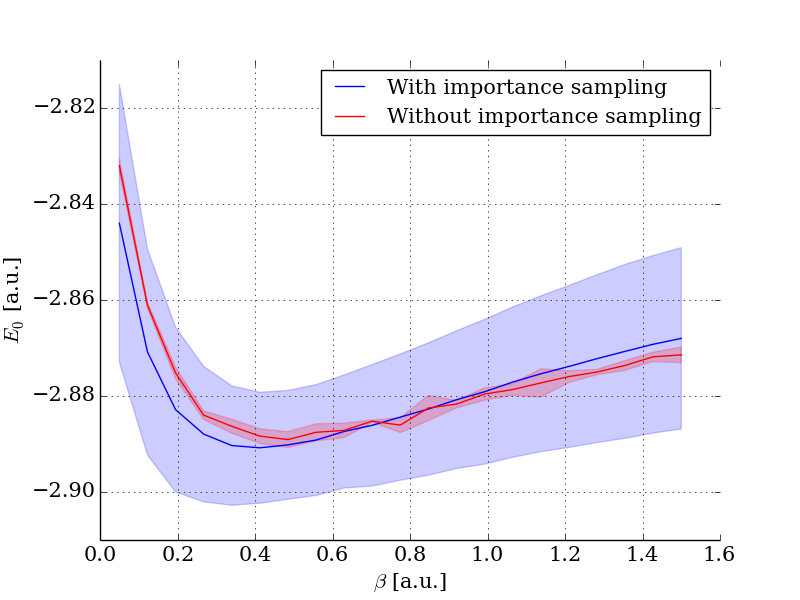
\includegraphics[width=\columnwidth]{../res/plot/helium_01/helium_01_pretty.png}
	\caption{}\label{fig:1}
\end{figure}

\section{Methods}
\subsection{The Quantum Mechanical System}
The Helium atom consists of two electrons orbiting a nucleus,
where the distance between electron 1 and the nucleus,
and electron 2 and the nucleus are labeled as
$r_1 = \sqrt{x_1^2 + y_1^2 + z_1^2}$ 
and $r_2 = \sqrt{x_2^2 + y_2^2 + z_2^2}$ in cartesian coordinates.

The total potential energy of the system is modelled as
{\small
\eq{
    V(r_1,r_2)=-\frac{2}{r_1}-\frac{2}{r_2}+\frac{1}{r_{12}}
}}%
where the interaction between each electron and the nucleus
is given by the two first terms. 
The mutual electron-electron repulsion is given by the last.
The distance between two electrons is $r_{ij}=|\vec r_j-\vec r_i|$.

The \textit{Hamiltonian} of the system is thus
\eq{
    \OP H = -\frac{\nabla_1 ^2}{2} -\frac{\nabla_2 ^2}{2}
    -\frac{2}{r_1}-\frac{2}{r_2}+\frac{1}{r_{12}}
}
scaled to \textit{atomic units} (a.u.).

This is based on the simplified, analytically solvable, system for the 
Hydrogen atom, where the Hamiltonian is
\equ{
  \OP H = \OP K + \OP V = -\frac{\hbar^2}{2m_e}\op \nabla^2 
  - \frac{e^2}{4\pi \epsilon_0 r} \label{eq:hydro}
}
with $e$ as the electron charge, $r$ is the radius from the proton to the electron
and $m_e$ as the mass of the electron.

This operator satisfies the \textit{time-independent Schr\"odinger Equation}
\equ{
  \OP H \ket{\psi} = E \ket{\psi}\label{eq:schrod}
}
where $E$ is the \textit{energy eigenvalue} and $\psi$ is the \textit{eigenstate} of the system.

For a Hydrogen-like quantum mechanical system, we can model the general
Hamiltonian of an atom as
\eq{
  \OP H
  &=\sum_i (\op k_i + \op v_i)  + \sum_{i<j} \op v_{ij}\\
  &= -\sum_{i=1}^N\bigg[
    \frac{\op\nabla_i^2}{2} + \frac{Z}{r_i}\bigg] 
  + \sum_{i=1}^{N-1}\sum_{j=i+1}^N\frac{1}{r_{ij}} \numberthis\label{ham}
}
Here $Z$ is the nuclear charge, 
and we have another sum for all the electron-electron repulsions.

We can add to this model by setting up a system of two atoms,
a \textit{diatomic molecule}, which gives us a Hamiltonian on the form
\eq{
  \OP H = -\sum_{i=1}^N\bigg[
    \frac{\op\nabla_i^2}{2} + \frac{Z_1}{r_{ip1}} + \frac{Z_2}{r_{ip2}}\bigg] 
    + \sum_{i=1}^{N-1}\sum_{j=i+1}^N\frac{1}{r_{ij}} + \frac{Z_1 Z_2}{R}
}

We now want to look at the form of the wave function for the Hydrogen atom.
The Hamiltonian (\ref{eq:hydro}) in atomic units is
\eq{
  \OP H = -\frac{\op \nabla^2}{2}- \frac{1}{r}
}

and the energy eigenvalues in (\ref{eq:schrod}) are given by
\eq{
  E_n = -\frac{1}{2n^2}
}

Solving the Schr\"odinger equation is done by separation of variables in
spherical coordinates
\equ{
  \psi_{nlm}(r,\theta,\varphi) = R_{nl}(r) Y_l^{m}(\theta,\varphi)\label{eq:psi}
}

where $n$, $l$ and $m$ are quantum numbers 
(principal, azimuthal and magnetic respectively).
The solution is separated into a radial part $R_{nl}$ and an angular part $Y_l^{m}$
called the spherical harmonics.
A large part of this project is using the solutions of the \textit{Hydrogen-like}
wave functions as basis for the wave function for Helium, Beryllium and Neon.

The solutions of the first few \textit{atomic orbitals} (and the ones we will use), 
are on the form
\eq{
  \psi_{100} &= \phi_{1s} =  e^{-\alpha r}\\
  \psi_{200} &= \phi_{2s} =  \left(1-\frac{\alpha r}{2}\right)e^{-\alpha r/2} \\
  \psi_{211} &= \phi_{2p_x} = x e^{-\alpha r/2}\\
  \psi_{210} &= \phi_{2p_y} = y e^{-\alpha r/2}\\
  \psi_{21-1}&= \phi_{2p_z} = z e^{-\alpha r/2}
}
where $x$, $y$ and $z$ are the cartesian coordinate positions of the electron,
and $\alpha$ is some charge.

\subsection{Slater Determinants}
The Hamiltonian (\ref{ham}) introduced in the last section is invariant
when you interchange two particles, and since electrons are \textit{fermions},
it is required that the wave function is antisymmetric.

In practice, this means that for a system of two particles, $1$ and $2$, described by the
wave functions $\psi_a$ and $\psi_b$, we must have a total wave function on the form
\equ{
  \psi^{1,2} = \psi_a^1 \psi_b^2 - \psi_b^1 \psi_a^2\label{wavfunc}
}
This is a result that follows from the fact that particles are indistinguishable,
and the minus sign comes from the antisymmetry condition.
An exchange operator $\OP P$ acting on an antisymmetric wave function,
will therefore change the sign, thus the wave function is an eigenfunction
of $\OP P$ with eigenvalue $p=-1$.

For bosons however, the sign is positive. This means that 
they do not obey the \textit{Pauli principle},
stating that two particles can not occupy the same state, 
which would imply $\psi^{1,2}=0$.

If we rewrite equation (\ref{wavfunc}), we see that this is actually a determinant
\eq{
  \psi^{1,2} = \vmat{\psi_a^1&\psi_b^1\\ \psi_a^2&\psi_b^2}
}
that can be generallized to the $N$-particle case as
\equ{
  \psi(\vec r_1, \dots, \vec r_n) 
  = \frac{1}{\sqrt{n!}}\vmat{\psi_1^1&\cdots&\psi_n^1\\ 
  \vdots & \ddots & \vdots \\ 
  \psi_1^n& \cdots &\psi_n^n}\label{slaterdet}
}
These Slater determinants obey exchange operations, since switching
two rows of the determinant changes the sign.
In our project we will omit the factor in front of the determinant,
as the important part is proportionality, and we will see later that constants get cancelled.

In this project, we are studying spin-$\frac{1}{2}$ particles,
and we must address this problem in the Slater determinants we will use.
The electrons have either spin $\uparrow$ or $\downarrow$,
so our determinant in (\ref{slaterdet}) 
have elements labeled $\uparrow$ or $\downarrow$.
However, we must also label them by their atomic orbitals,
so an element of the determinant will have the form
\eq{
  \phi_{j\sigma}(\vec r_i) = \phi_{j\sigma}^i
}
where $j$ is the atomic orbital (1s, 2s, 2p in this project), $\sigma$ is the spin,
and $i$ is the particle number.
Determinants of matrices with elements like that for Helium, Beryllium and Neon, 
are unfortunately zero, 
since they are independent of spin
(two and two columns would be equal).
This can be bypassed by writing the determinant $\abs*{\op D}$ as a product of two smaller ones
for each spin\footnote{Ref. [1], p. 519-520}, since
\equ{
  \psi_D = \abs*{\op D} \propto \abs*{\op D}_{\uparrow} \abs*{\op D}_{\downarrow}
  \label{eq:det}
}
By doing this, the wave function
will lose its antisymmetry when interchanging particles,
but it doesn't affect the expectation values.

For Helium,
we write the wave function as a product of the (reduced) $1\times1$ matrices
to simplify the function. Therefore
\eq{
  \psi_D^{He} = \phi_{1s}(\vec r_1) \phi_{1s}(\vec r_2)
}

For Beryllium (four electrons), the corresponding Slater determinant is
\equ{
  \psi_D^{Be} 
    &=\vmat{
    \phi_{1s\uparrow}^1&\phi_{1s\uparrow}^2
      &\phi_{1s\uparrow}^3&\phi_{1s\uparrow}^4\\
    \phi_{1s\downarrow}^1&\phi_{1s\downarrow}^2
      &\phi_{1s\downarrow}^3&\phi_{1s\downarrow}^4\\
    \phi_{2s\uparrow}^1&\phi_{2s\uparrow}^2
      &\phi_{2s\uparrow}^3&\phi_{2s\uparrow}^4\\
    \phi_{2s\downarrow}^1&\phi_{2s\downarrow}^3
      &\phi_{2s\downarrow}^2&\phi_{2s\downarrow}^4
    }\\
    &=\vmat{
    \phi_{1s\uparrow}^1&\phi_{1s\uparrow}^2\\
    \phi_{2s\uparrow}^1&\phi_{2s\uparrow}^2\\
    }
    \vmat{
    \phi_{1s\downarrow}^3&\phi_{1s\downarrow}^4\\
    \phi_{2s\downarrow}^3&\phi_{2s\downarrow}^4\\
    }\label{eq:bespin}
}
and finally for Neon (ten electrons), 
the spin $\uparrow$ part
\equ{
  \abs*{\op D}_{\uparrow}^{Ne} 
    &=\vmat{
    \phi_{1s\uparrow}^1&\phi_{1s\uparrow}^2
      &\phi_{1s\uparrow}^3&\phi_{1s\uparrow}^4&\phi_{1s\uparrow}^5\\
    \phi_{2s\uparrow}^1&\phi_{2s\uparrow}^2
      &\phi_{2s\uparrow}^3&\phi_{2s\uparrow}^4&\phi_{2s\uparrow}^5\\
    \phi_{2p_x\uparrow}^1&\phi_{2p_x\uparrow}^2
      &\phi_{2p_x\uparrow}^3&\phi_{2p_x\uparrow}^4&\phi_{2p_x\uparrow}^5\\
    \phi_{2p_y\uparrow}^1&\phi_{2p_y\uparrow}^2
      &\phi_{2p_y\uparrow}^3&\phi_{2p_y\uparrow}^4&\phi_{2p_y\uparrow}^5\\
    \phi_{2p_z\uparrow}^1&\phi_{2p_z\uparrow}^2
      &\phi_{2p_z\uparrow}^3&\phi_{2p_z\uparrow}^4&\phi_{2p_z\uparrow}^5
    }\label{eq:nespinup}
}
and similarly for $\downarrow$
\equ{
  \abs*{\op D}_{\downarrow}^{Ne} 
    &=\vmat{
    \phi_{1s\uparrow}^6&\phi_{1s\downarrow}^7
      &\phi_{1s\downarrow}^8&\phi_{1s\downarrow}^9&\phi_{1s\downarrow}^{10}\\
    \phi_{2s\downarrow}^6&\phi_{2s\downarrow}^7
      &\phi_{2s\downarrow}^8&\phi_{2s\downarrow}^9&\phi_{2s\downarrow}^{10}\\
    \phi_{2p_x\downarrow}^6&\phi_{2p_x\downarrow}^7
      &\phi_{2p_x\downarrow}^8&\phi_{2p_x\downarrow}^9&\phi_{2p_x\downarrow}^{10}\\
    \phi_{2p_y\downarrow}^6&\phi_{2p_y\downarrow}^7
      &\phi_{2p_y\downarrow}^8&\phi_{2p_y\downarrow}^9&\phi_{2p_y\downarrow}^{10}\\
    \phi_{2p_z\downarrow}^6&\phi_{2p_z\downarrow}^7
      &\phi_{2p_z\downarrow}^8&\phi_{2p_z\downarrow}^9&\phi_{2p_z\downarrow}^{10}
    }\label{eq:nespindown}
}

Here we have used equality instead of proportionality, since these are the actual
wave functions we will use.

\subsection{The Variational Principle}
The Variation Principle states that if we have a Hamiltonian
$\OP H$ and a trial wavefunction $\psi_{T}$,
an upper bound for the ground state energy $E_0$ is given by
equation (\ref{E0var}). 
\equ{
	E_0 \leq
	\langle H \rangle =
	\frac{\Int{}{}{\vec R}{\psi_T^*(\vec R) \OP{H}(\vec R) \psi_T(\vec R)}}
	{\Int{}{}{\vec R}{\psi_T^*(\vec R) \psi_T(\vec R)}}\label{E0var}
}
To find such a wave function, we expand it in the eigenstates of
the Hamiltonian (since they form a complete set) as follows
\eq{
  \psi_T(\vec R) = \sum_i c_i \psi_i(\vec R)
}
and given that they are normalized, we get
\eq{
  E_0 \leq
  \frac{\sum_{i,j}c_m^*c_n\Int{}{}{\vec R}{\psi_m^*(\vec R) \OP{H}(\vec R) \psi_n(\vec R)}}
	{\sum_{m,n}c_m^*c_n\Int{}{}{\vec R}{\psi_m^*(\vec R) \psi_n(\vec R)}}\label{E0var}
  = \frac{\sum_n \abs*{c_n}^2 E_n}{\sum_n \abs*{c_n}^2}
}
since $E_0 = E_0 \sum_n \abs*{c_n}^2 \leq \sum_n E_n \abs*{c_n}^2 $

The key to the variational principle is to find suitable trial wave functions
that live in the same Hilbert space as the Hamiltonian.
Given a trial wave function, we can then vary som parameters 
$\vec \alpha = (\alpha,\,\beta,\,\dots)$ to optimalize the function,
and the energy value $E_T$.

Another (analytical) quantity that we want to calculate, is the \textit{local energy}
\begin{equation}
  E_L(\vec R, \vec \alpha) = \frac{1}{\psi_T(\vec R, \vec \alpha)} \OP H \psi_T(\vec R, \vec \alpha)\label{eq:local}
\end{equation}
which together with (\ref{E0var}) yields
\begin{equation}
  \langle H \rangle 
  = \frac{\Int{}{}{\vec R}{E_L \abs*{\psi_T}^2}}
	{\Int{}{}{\vec R}{\abs*{\psi_T}^2}} \label{exp}
\end{equation}

\subsection{Variational Monte Carlo (VMC)}
The integrals to be solved in the variational method,
does not scale well with traditional integral methods when 
increasing the number of particles and dimensions and using 
more complex wave functions .
Therefore, we introduce the \textit{brute-force Monte Carlo method}
to solve the integrals.

We define
\eq{
  P(\vec R) \equiv \frac{\abs*{\psi_T}^2}{\Int{}{}{\vec R}{\abs*{\psi_T}^2}}
}
and can then rewrite the integral in (\ref{exp}), and approximate it as
\eq{
  \Int{}{}{\vec R}{E_L P(\vec R)} \approx \frac{1}{N}\sum_{i=1}^N E_L P(\vec R)
}
Here $N$ is the number of \textit{Monte Carlo samples}.
An outline of the algorithm can be seen in Algorithm \ref{algo:vmc}.

\begin{algorithm}[H]
	\caption{VMC Algorithm}\label{algo:vmc}
  \begin{algorithmic}[1]
    \Procedure{Initialization}{}
      \State{Set a fixed number of MC steps.}
      \State{Choose initial position $\vec R$ and variational
            
            parameters $\boldsymbol\alpha$.}
      \State{Calculate $|\psi_T(\vec R)|^2$.}
    \EndProcedure
    \Procedure{Initialize energy and variance and start the MC calculation}{}
      \State{Find the trial position $\vec R' =\vec R + \delta\times r $,
      
            where $r\in [0,1]$ is randomly selected.}
      \State{Use the Metropolis algorithm to determine if the
      
            move $w =\frac{P(\vec R')}{P(\vec R)}$ is accepted or rejected.}
      \State{Given that the move is accepted, set $\vec R = \vec R'$.}
      \State{Update averages.}
    \EndProcedure
    \Procedure{Compute final averages}{}
    \EndProcedure
  \end{algorithmic}
\end{algorithm}

\subsection{The Metropolis Algorithm}
In the VMC algorithm (Algorithm \ref{algo:vmc}),
one of the steps is to perform the Metropolis algorithm to determine wheter or not
a step is rejected or accepted.

The Metropolis algorithm samples a normalized probability distribution
by a stochastic process. In other words, it is a method for simultaing
random walks, which we can use to do brute-force Monte Carlo computations.
The algorithm uses \textit{Markov chains}, where each state $i$,
has some probability of going to another state $j$.
Each state is only dependent on the last state it was in.

Define $P^{(n)}_i$ as the probability for finding the system in state $i$
at some step $n$. This probability is given by the sum of the probability of
previously being in a state $j$, transitioning to $i$, $T_{j\rightarrow i}$,
and the probability of rejecting the transition to another state $j$,
$1-A_{i\rightarrow j}$.
Where $A$ is the acceptance ratio

This results in
\eq{
  P_{i}^{(n)} = 
  \sum_j \left[
  P_{j}^{(n-1)} T_{j\rightarrow i} A_{j\rightarrow i}-
  P_{i}^{(n-1)} T_{i\rightarrow j} A_{i\rightarrow j}
  \right]
}
since the probability of making a transition must be $1$, $\sum_j T_{i\rightarrow j}$.


See Algorithm \ref{algo:metro} for an outline of the Metropolis algorithm.

\begin{algorithm}[H]
	\caption{Metropolis Algorithm}\label{algo:metro}
  \begin{algorithmic}[1]
    \Procedure{Metropolis test}{}
      \State{Sample a possible new state $j$,
       
      with a probability $T_{i\rightarrow j}$.}
      \State{With probability $A_{i\rightarrow j}$, accept $j$ as a new state.}
      \State{Set it as the new sample.}
      \State{The move is rejected with probability $1-A_{i\rightarrow j}$.}
      \State{Set $i$ as the sample again.}
    \EndProcedure
  \end{algorithmic}
\end{algorithm}

\subsection{Importance Sampling}
A random walker is the most efficient way to sample where the
wave function is large. To further increase the efficiency, we can implement importance
sampling, where the walk in space is governed by the trial wave function.
The idea is to try and drive the walker in to an area with a higher probability
density.

In the brute force method, one tries a new position
\eq{
  y = x + \xi \sqrt{\Delta t}
}
where $\xi$ a \textit{gaussian random variable} centered on $x$.
With importance sampling, we add a term that takes into consideration
where the probability density is higher.

The results are based on the 
\textit{Fokker-Planck equation} and the \textit{Langevin 
equation}. This makes the step look similar to a diffusion process,
where the new position is given by
\begin{align*}
y = x + DF(x) \delta t + \xi \sqrt{\Delta t}.
\end{align*}

In this equation, $\xi $ is a gaussian random variable 
and $\Delta t$ is a chosen time step.
In atomic units, $D$ is $1/2$, and in our plots $\Delta t = 0.01$. 

An important part of this result is that the walker is affected by $F(x)$
which contains the trial wavefunction. This force has been named 
the \textit{quantum force}, given by
\begin{align*}
\vec F = 2\frac{1}{\psi_T}\nabla \psi_T. 
\end{align*}

This also has the result of changing the random number check in the 
Metropolis algorithm from:
$q(y,x) = |\psi_T(y)|^2/|\psi_T(x)|^2$ to: 
\[
q(y,x) = \frac{G(x,y,\Delta t)|\psi_T(y)|^2}{G(y,x,\Delta t)|\psi_T(x)|^2}.
\]

Where G is the Green function given by
\eq{
  G(y,x,\Delta t) =  \frac{1}{(4\pi D\Delta t)^{3N/2}}\\ \cdot \exp{\left(-(y-x-D\Delta t F(x))^2/4D\Delta t\right)}.
}
This has its basis in our change of center for the gaussian distribution.

\subsection{Statistical Analysis}
The MC calculations are a set of computational \textit{experiments} 
with statistical errors. In these experiments, we are interested in the mean
value of the ground energies and the density distribution. The 
individual samples are not as interesting to us, and we would rather like
to look at the variance of the mean values. 
The variance of the mean value is closely connected with the correlation
in the individual samples. 

%This can be shown mathematically, but the result
%is this
%\eq{
%  \sigma^2(m) &= \frac{1}{n^2}\sum_{i,j=1}^{n} \mathrm{Cov}(x_i,x_j)
%}

Both our random walker with and without importance sampling, gives correlated
samples. In our case, we use \textit{blocking}\footnote{Ref. [2], p. 60-61}
as a technique to find out have many steps
the walker has to do to be as uncorrelated as possible in comparison with its first step.
This means that for a set of random samples $A$, one sample $A_i$ will be correlated
to some other sample $A_{i+n}$.

If we we group our data ($N$ samples) in blocks of size $n_b$,
then the number of blocks is $m = N/n_b$.
The average of one block $i$ (the average of all samples
between $i n_b + 1$ and $(i+1)n_b$), is given by 
\eq{
\langle A \rangle_i = \frac{1}{n_b}\sum_{j=in_b+1}^{(i+1)n_b} A_j
}

We can then calculate the average of all the blocks as
\eq{
  \langle A \rangle = 
  \frac{1}{m}\sum_{i=1}^m \left(
    \frac{1}{n_b}\sum_{j=in_b+1}^{(i+1)n_b} A_j \right)
  \equiv \frac{1}{m}\sum_{i=1}^m \langle A \rangle_i
}
and the variance as
\eq{
  \Var{A}=
  \frac{1}{m}\sum_{i=1}^m \langle A \rangle_i^2
  -\left(\frac{1}{m}\sum_{i=1}^m \langle A \rangle_i\right)^2
}

By plotting the variance of the mean as a function of block size we 
will see that it reaches a plateau.
This plateau means that increasing the sample length will no longer
change the variance in the mean significantly. 
This happens at some block size $n_b > K_0$, 
where $K_0$ is called the \textit{correlation length}. 
This makes us able to more easily calculate variance in the mean because we know how small block sizes we can use. 
This is used to make the standard deviation interval around our density plots. 

\begin{algorithm}[H]
	\caption{Blocking Method}\label{algo:block}
  \begin{algorithmic}[1]
    \Procedure{Compute variance of mean}{}
      \State Compute MC calculation, store samples in array.
      \State Loop over a set of block sizes $n_b$.
      \State For each $n_b$, calculate the mean of the block,
      
        and store these values in a new array.
      \State Take the mean and variance of this array.
      \State Store results.
    \EndProcedure
  \end{algorithmic}
\end{algorithm}

\subsection{The Hydrogen-Like Trial Wave Functions}
The arguably most important part of the project is to find good
trial wave functions. In the following, we will present
the wave functions we have used in this project.
In this section, we show the functions which are based on
the solutions of (\ref{eq:psi}).

Our trial wave function is a product of the Slater determinant $\psi_D$ and
a correlation part $\psi_C$ that considers the electron-electron repulsion.
The second part is also called the \textit{Jastrow factor}\footnote{Ref. [2], p. 280}.
The the general trial wave function is
\eq{
  \psi_T = \psi_D \psi_C
}
The trial wave functions are always dependent on the coordinates of every
electron in some way.
The Jastrow factor is generally written as
\equ{
  \psi_C = \prod_{i<j}^{n}\exp{\left(\frac{a r_{ij}}{1+\beta r_{ij}}\right)}
  \label{eq:psicor}
}
where $a$ is a factor that takes into account the spin of electron $i$ and $j$,
the \textit{electron-electron cusp conditions}.
When the particles have equal spin we have $a=\sfrac{1}{4}$,
and when they are different $a=\sfrac{1}{2}$ (for example the ground state of Helium).
For Beryllium and Neon, we set the spin of the first $\sfrac{n}{2}$ particles to
$\uparrow$ and the last half to spin $\downarrow$.
The Slater determinant part is given by (\ref{eq:det}).

We also want to determine the local energy $E_L$ to approximate
the ground state energy of the atom.
The general expression for the local energy is
\eq{
  E_L = \frac{1}{\psi_T (\vec R)}\OP H \psi_T (\vec R) 
}
and the Hamiltonian can generally be described as in (\ref{ham}).

From this expression, it's clear that $\OP K$ is the only operator that changes the
trial wavefunction when we calculate the local energy. Therefore, we must calculate the
following quantities
\eq{
  \frac{1}{\psi_T}\op k_i \psi_T = -\frac{1}{2}\frac{\op\nabla_i^2 \psi_T}{\psi_T}
}
The product rule of differentiation gives us
\eq{
  \frac{\op\nabla^2 \psi_T}{\psi_T} = 
  \frac{\op\nabla^2 \psi_D}{\psi_D}
    +2 \frac{\op\nabla \psi_D}{\psi_D}\cdot\frac{\op\nabla \psi_C}{\psi_C}
    +\frac{\op\nabla^2 \psi_C}{\psi_C}
}
So we need to calculate the four quantities
\eq{\mat{
  \frac{\op\nabla^2 \psi_D}{\psi_D}&
    \frac{\op\nabla \psi_D}{\psi_D}&
    \frac{\op\nabla \psi_C}{\psi_C}&
    \frac{\op\nabla^2 \psi_C}{\psi_C}
}}
They are derived in the appendix, and they are not only useful when calculating the
local energy, which we will see in the implementation section.

\subsubsection{The First Trial Wave Function of Helium}
We first model the variational solution with a trial function of one
variation parameter $\alpha$ 
(corresponding to the $\alpha$ in Hydrogen solution(\ref{eq:psi})).
It has the form
\eq{
\psi_{T1}^{He}({\bf r_1},{\bf r_2}) = 
   \exp{\left(-\alpha(r_1+r_2)\right)}
}
which is the Slater-determinant part of the wave function.

We now proceed to find the local energy, given by (\ref{eq:local}).
The only part of the operator $\OP H$ from (\ref{ham}) that affects the wave function
are the Laplace operators.
Since $\psi_{T1}$ is only spatially dependent on $r_1$ and $r_2$, we have
\eq{
  \nabla_i^2 \psi_{T1}^{He} = \bigg( \frac{\partial^2}{\partial r_i^2} 
    + \frac{2}{r_i} \frac{\partial}{\partial r_i} \bigg) \psi_{T1}^{He}
    = \bigg( \alpha^2 -\alpha\frac{2}{r_i}  \bigg)\psi_{T1}^{He}
}
for $i = 1,\;2$, since

\eq{
  \frac{\partial}{\partial r_i} e^{-\alpha (r_1+r_2)}
    &= -\alpha e^{-\alpha (r_1+r_2)}\\
\frac{\partial^2}{\partial r_i^2} e^{-\alpha (r_1+r_2)}
    &= \alpha^2 e^{-\alpha (r_1+r_2)}
}
This gives us the following trial energy

\eq{
  E_{L1}^{He}
  &=(\alpha-2)\bigg( \frac{1}{r_1}+\frac{1}{r_2} \bigg)
    +\frac{1}{r_{12}}-\alpha^2
}
The $2$ in the $\alpha-2$ term is the number of protons, $Z$.

\subsubsection{The second trial wavefunction}
To approximate the closed-form solution even better,
we assume another trial wavefunction based on the fact that
the two electrons interact, namely
\eq{
  \psi_{T2}^{He} (\vec r_1,\vec r_2)
    =\exp{\left(-\alpha(r_1+r_2)\right)}
    \exp{\left(\frac{r_{12}}{2(1+\beta r_{12})}\right)}
}

One can then in the same way as for $\psi_{T1}$ calculate
the local energy. The correlations part will give us some trouble
when we try to calculate the Laplacian. This is due to
the distance between $\vec r_1$ and $\vec r_2$, since this quantity
is dependent on the angles $\varphi$ and $\theta$.
The local energy now has the form
\eq{
	E_{L2}^{He} = E_{L1}^{He}&+\frac{1}{2(1+\beta r_{12})^2}
	\bigg(\frac{\alpha(r_1+r_2)}{r_{12}}(1-
	\frac{\mathbf{r}_1^T\mathbf{r}_2}{r_1r_2})\\
	&-\frac{1}{2(1+\beta r_{12})^2}-\frac{2}{r_{12}}+
	\frac{2\beta}{1+\beta r_{12}}\bigg)
}

\subsubsection{Cusp Conditions}
As mentioned earlier, our trial wave function should behave as much
as the exact wave function as possible.
This means that there are some criteria that must be fulfilled.
One of these is that the wave function and its derivative
should be well defined at the origin,
so that $\psi_T(\vec R = 0)\neq 0$.
For Helium, we have a radial symmetry, so the angular terms go away.
Then we have $\psi_T = \psi_T^r$ where the $r$ stands for \textit{radial}.

Assuming that the two electrons are far apart, and $r_2 \neq 0$,
we let $r_1 \rightarrow 0$. Then the local energy is
\eq{E_L &=
  \frac{1}{\psi_T^{r}}\left( -\frac{1}{2}\frac{\mathrm d^2}{\mathrm d r_1^2}
  - \frac{1}{r_1}\frac{\mathrm d}{\mathrm d r_1} - \frac{Z}{r_1} + \text{f.t.}
  \right)\psi_T^{r}\\
  \lim_{r_1\rightarrow 0} E_L &=\frac{1}{\psi_T^{r}(r_1)}
  \left(- \frac{1}{r_1}\frac{\mathrm d}{\mathrm d r_1} 
  - \frac{Z}{r_1}\right)\psi_T^{r}(r_1)
}\footnote{f.t. here stands for \textit{finite terms}}
The second derivative does not diverge due to the finiteness condition.
FOr $l=0$, we then have differential equation
\eq{
  \frac{1}{\psi_T^{r}(r_1)}\frac{\mathrm d \psi_T^{r}(r_1)}{\mathrm d r_1}
  = -Z
}
with solution $\psi_T^{r}(r_1) \propto \exp(-Zr_1)$, and similarly for $r_2$.
For $l>0$, the $-Z$ turns into $\sfrac{-Z}{(l+1)}$.\footnote{Ref. [1], p. 477-478}

When the two electrons approavh each other, we have $r_{12}\rightarrow 0$.
The radial equation is the same in this case, with the attraction
switched with the electron-electron repulsion, and the kinetic energy is twice as large.
We get
\eq{
  \lim_{r_{12}\rightarrow 0} E_L &=\frac{1}{\psi_T^{r}(r_{12})}
  \left(
  \frac{4}{r_{12}}\frac{\mathrm d}{\mathrm d r_1} + \frac{2}{r_{12}}
  \right)\psi_T^{r}(r_{12})
}
The solution for the differential equation when $l=0$
\eq{
  \frac{1}{\psi_T^{r}(r_{12})}\frac{\mathrm d \psi_T^r(r_{12})}{\mathrm d r_1} = -2
}
is $\psi_T^r(r_{12}) \propto \exp(-r_{12}/2)$.

\subsubsection{Beryllium}
The trial wavefunction of Beryllium can be written as a product of a Slater determinant
part and a correlation part on the form
\equ{
  \psi_{T}(\vec r_1, \vec r_2, \vec r_3, \vec r_4) = \psi_{D}\psi_{C} \label{psiT}
}
where the Slater determinant is
\equ{
  \psi_D &= Det\left(\phi_{1}(\vec r_1),\phi_{2}(\vec r_2),
    \phi_{3}(\vec r_3),\phi_{4}(\vec r_4)\right) \label{psiD}\\
  &= \left(\phi_{1s}^1\phi_{2s}^2
    -\phi_{1s}^2\phi_{2s}^1\right)
    \left(\phi_{1s}^3\phi_{2s}^4
    -\phi_{1s}^4\phi_{2s}^3\right)\nonumber
}
and the correlation part is
\equ{
  \psi_C = \prod_{i<j}^{4} g_{ij}
   =\prod_{i<j}^{4}\exp{\left(\frac{ar_{ij}}{1+\beta r_{ij}}\right)} \label{psiC}
}
Here $\phi_i(\vec r_i)$ are the hydrogen-like wavefunctions. They are given by
the $1s$ and $2s$ orbital parts
\eq{                                                               
  \phi_{1s}^i &= e^{-\alpha r_i}\\
  \phi_{2s}^i &= \left(1-\alpha r_i/2\right)e^{-\alpha r_i/2}
}
which are dependent on the cartesian positions $\vec r_i = (x_i,y_i,z_i)$. 
The relative distance between two particles is
\eq{
  r_{ij} &= \abs{\vec r_j - \vec r_i} 
  \\&= \sqrt{(x_j-x_i)^2+(y_j-y_i)^2+(z_j-z_i)^2}
}
and obviously $r_{ij}=r_{ji}$.

\subsubsection{Neon}
For Neon, in addition to $$ $$ we need three more hydrogenic wavefunctions for the $2p$ orbital, given by
$2p_x$, $2p_y$ and $2p_z$. These are given by

\eq{
  \phi_{2p_k}(\vec r_i) &= \alpha k_i g_i \text{ for } k_i = x_i,y_i,z_i
}
so the wave function is
\eq{
  \psi_T^{Ne} = |\op D|\uparrow|\op D|\downarrow
  \prod_{i<j}^{10}\exp{\left(\frac{a r_{ij}}{1+\beta r_{ij}}\right)}
}
where the two Slater determinants are given in (\ref{eq:nespinup})
and (\ref{eq:nespindown}).

\subsection{Introducing Gaussian-Type Orbitals}
In this project, we have shown how one can use Hydrogen-like wave functions as the basis
for the Slater determinant, and up until now, 
we have used so-called \textit{Slater-Type Orbitals} (STOs).
We will now replace the STOs with \textit{Gaussian-Type Orbitals} (GTOs).

The spin-factorized Slater determinants (one for spin up and one for spin down),
are given by
\eq{\psi_{D_{spin}} = 
  \vmat{\phi_1(\vec r_1)& \cdots & \phi_1(\vec r_n)\\
  \vdots&\ddots&\vdots\\
  \phi_n(\vec r_1)& \cdots & \phi_n(\vec r_n)}
}

where $n$ is equal to half the number of particles, 
and  $\phi_j(\vec r_i)$ are one-particle wave functions 
$\phi_{1s}$, $\phi_{2s}$ and $\phi_{2p(3)}$
($(3)$ is short-hand notation for the $x$, $y$ and $z$ parts).
These spin independent, one-particle wave functions are
linear combinations of basis functions, and we will now use \textit{contracted} GTOs
(CGTOs) for this purpose.

The functions can then be written as
\equ{\phi_j(\vec r_i) = \sum_p C_{pj} \varphi_p(\vec r_i)\label{eq:gto}
}

The CGTOs are on the form
\eq{
  \varphi_p^{CGTO}(\vec r_i) = \sum_k N_k \varphi^{GTO}_k(\vec r_i)
}
with
\eq{
  \varphi^{GTO}_k = d_k x^m y^n z^o e^{-\alpha_k r^2}
}
which are called \textit{cartesian} GTOs. 
The numerical coefficients $\alpha_k$ and $d_k$ are chosen to optimalize the
basis functions.

The normalization factors are given as\footnote{Ref. [2], p. 280}
\eq{
  N_k = \left(\frac{2\alpha_k}{\pi}\right)^{3/4}
  \sqrt{\frac{(4\alpha_k)^{m+n+o}}{(2m-1)!!(2n-1)!!(2o-1)!!}}
}
and since they are dependent on the total angular momentum,
given by the quantum numbers $l = m+n+o$, we will write them as
$N_k = N_{m,n,o}$.

\subsection{Nonlinear Conjugate Gradient Method}
Our aim is to calculate the lowest mean of the ground state energy $E_0$,
but it depends on some variational parameters $\vec \alpha$.
Therefore we need to find the global minimum with respect to these parameters,
where
\eq{
  \frac{\partial E}{\partial \alpha_i} = 0
}
where $\alpha_i$ can take the values $\alpha$ and $\beta$.

For a function $f$ that we wish to minimize, with
\eq{
  f(x) = \frac{1}{2}x^T Ax + b^Tx + c
}
we use the \textit{nonlinear conjugate gradient method} 
(NGC)\footnote{Ref. [5] p. 120-122}
to do it, see Algorithm \ref{algo:ngc}.
We proceed one step, decided by $x_{k+1}=x_k + ad_k$, where $a$
is the step. This step is decided by \textit{line search method},
for example the \textit{bisection method} (outlined in Algorithm \ref{algo:bisec}).
The search is guided by the direction $d_k$.


\begin{algorithm}[H]
	\caption{NCG method}\label{algo:ngc}
  \begin{algorithmic}[1]
    \Procedure{Initialize}{}
      \State{Let $k=0$ and $x_k=x_0$ be our initial guess.}
      \State{Compute $d_k=d_0=-\nabla f(x_0)$.}
    \EndProcedure
    \Procedure{Find the best step size}{}
      \State{Compute $a$ to minimize $f(x_k+ a d_k)$
      
      by a line search in the direction $d_k$.}
    \EndProcedure
    \Procedure{Update current guess}{}
      \State{Let $x_{k+1}=x_k + ad_k$.}
    \EndProcedure
    \Procedure{Update the seacrh direction}{}
      \State{Let $d_{k+1} = -\nabla f(x_{k+1} + \beta_k d_k)$ where 
      \eq{\beta_k = \frac{\nabla f(x_{k+1}^T)(\nabla f(x_{k+1}-\nabla f(x_{k}))}
      {d_k^T(\nabla f(x_{k+1})-\nabla f(x_{k}))}}}
    \EndProcedure
    \Procedure{Iterate}{}
      \State{Repeat procedures 2 to 4 until we have looked in all 
      
      directions ($\dim x$).}
    \EndProcedure
  \end{algorithmic}
\end{algorithm}

Given a function $g(x)$ and an interval $[a,b]$, where $g(a)$ and $g(b)$
has opposite signs (at least one zero crossing),
we want to find the minimum.
Calculate $f(c)$ for $c = \sfrac{(a+b)}{2}$, if $f(c)$ has opposite
sign of $f(a)$ ($f(b)$) then the minimum is in $[a,c]$ ($[c,b]$).
Choose the new interval and continue until minimum is found (for some tolerance).

\begin{algorithm}[H]
	\caption{Bisection method}\label{algo:bisec}
  \begin{algorithmic}[1]
    \Procedure{Iteration}{}
      \While{$n<N_{max}$}
        \State{Compute $c$ and $f(c)$.}
        \State{If minimum is found, return $c$. Success.}
        \State{If not: choose new interval $[a,c]$ or $[c,b]$.}
      \EndWhile
    \EndProcedure
  \end{algorithmic}
\end{algorithm}

\clearpage




\section{Implementation}
The methods described above are implemented in an object oriented C++ program
which is simple to use, and does not have any dependencies. 

Most of the code is contained in the class VMCSolver.cpp and VMCSolver.h. 
These were created to contain the full system and parameters for a single run. 

To start a simulation one must instantiate the solver and 
initialize the system, either by file and/or manually. After this
the integration can be run and all data will be contained in the solver object.
The last step is to collect data from the solver. 

All plot data are generated by individual programs using the mentioned solver. 
Plots are generated using python. 

\subsection{Efficient Computation of the Slater Determinant}

For larger atoms, the evaluation of the gradient and the Laplacian of the Slater
determinant becomes increasingly numerically demanding
to compute. Computing these quantities with brute force, 
leads to $N\cdot d$ operations to find the determinant and thus
multiplying this with our $O(N^3)$ operations.
In the following, we derive a method that deals with this issue, 
and achieves a lower number of operations.

We can approximate the Slater determinant as
\eq{
	\Phi(\vec r_1, ..., \vec r_N) \propto \det\uparrow\cdot\det\downarrow
}
where the spin determinants are the determinants which only depend on spin up and spin down
respectively. The determinants are $2\times 2$ for Berylllium and $5\times 5$ for Neon.
This is true only if $\OP H$ is spin independent.

Then, $\det \op D = |\op D| = |\op D|_{\uparrow}\cdot |\op D|_{\downarrow}$, 
where the Slater matrices are dependent on the positions of the electrons. 
Each time we update the positions and differentiate the Slater determinant,
the Slater matrix is changed, but by calculating the determinant 
from scratch each time, we will certainly do unnecessary computations. 

This is solved by the following algorithm, that instead of calculating 
the determinant, updates the \textit{inverse} of the Slater matrix suitably.

We first express $(i,j)$ elements of the inverse of $\op D$ as
\eq{
  d_{ij}^{-1} = \frac{C_{ji}}{|\op D|}
}
where $C_{ji}$ is the transposed cofactor-matrix element of $\op D$.

This motivates the ratio
\eq{
  R \equiv \frac{|\op D(\vec r^{new})|_{\uparrow}}{|\op D(\vec r^{old})|_{\uparrow}} 
  = \frac{\sum_{j=1}^N d_{ij}^{new} C_{ij}^{new}}
    {\sum_{j=1}^N d_{ij}^{old} C_{ij}^{old}}
}
Every time we move particle $i$, the $i$-th row of $\op D$ changes,
and we have to update the inverse. However, the $i$-th row of $\op C$
is independent\footnote{Since the cofactor-matrix elements $c_{ij}$ is defined by 
removing $i$-th row and $j$-th column from a matrix $\op A$,
and then taking the determinant of the remaining matrix.} 
of the $i$-th row of $\op D$, which means that
we must have
\eq{
  \op C_{ij}^{new} = \op C_{ij}^{old} = (d_{ji}^{-1})^{old}\cdot |\op D| 
    \text{ for } j=1,...,N
}
and using
\eq{
  \sum_{k=1}^N d_{ik}\ d_{kj}^{-1} =\delta_{ij}
}
The result is
\eq{
  R=\sum_{j=1}^N d_{ij}^{new} (d_{ji}^{-1})^{old}
    =\sum_{j=1}^N \phi_j(\vec r_i^{new})\ d_{ji}^{-1} (\vec r_i^{old})
}

The algorithm for updating the inverse of the matrix 
when a new position is accepted is then

\begin{algorithm}
	\caption{Inverse of Slater Matrix}\label{algo1}
  \begin{algorithmic}[1]
    \Procedure{Update columns $j\neq i$}{}
    \For{each column $i\neq j$}
      \State{$ S_j = \sum_{l=1}^N d_{il}(\vec r^{new}) d_{lj}^{-1}(\vec r^{old}) $}
      \State{$ (d_{kj}^{-1})^{new} 
        = (d_{kj}^{-1})^{old} - \frac{S_j}{R}(d_{ki}^{-1})^{old} $} 
    \EndFor
    \EndProcedure
    \Procedure{Update column $i$}{}
      \State{$ (d_{ki}^{-1})^{new} 
        = \frac{1}{R}(d_{ki}^{-1})^{old} $}
    \EndProcedure
  \end{algorithmic}
\end{algorithm}

We can then calculate the gradient and laplacian as
\eq{
  \frac{\op\nabla_k |\op D|}{|\op D|} 
    = \sum_{j=1}^N \nabla_k \phi_j(\vec r_i^{new})\ d_{ji}^{-1} (\vec r_i^{old})\\
  \frac{\op\nabla_k^2 |\op D|}{|\op D|} 
    = \sum_{j=1}^N \nabla_k^2 \phi_j(\vec r_i^{new})\ d_{ji}^{-1} (\vec r_i^{old})
}

The time consuming part of the computation of the Slater determinant,
is calculating the Laplacian and gradient. This makes the
number of operations go from the already undesirable $\mathcal O(N^3)$ to
$\mathcal O(d\times N^4)$, since there are $d\times N$ independent coordinates.
Using the method above, the total calculation scales as
$\mathcal O(d\times N^2)$.


\subsection{Derivatives of the Trial Wave Functions}
In many of our calculations we need the Laplacian of the trial wave function,
divided by the wave function, or the gradients of the trial wave function.
In Appendix A, we have listed and (derived some of) these quantities,
but the implementation of the derivatives of
the Jastrow factor in the efficient Slater method, needs to be mentioned.

The Jastrow factor is given by
\equ{
  \psi_C = \prod_{i<j}^{n}\exp{\left(\frac{a r_{ij}}{1+\beta r_{ij}}\right)}
  \label{eq:psicor}
}
the gradient is
\eq{
  \frac{\op\nabla_k\psi_C}{\psi_C} =\sum_{i\neq k}\frac{\vec r_{ik}}{r_{ik}}\frac{a}{(1+\beta r_{ik})^2} 
}
and the Laplacian
{\tiny\begin{equation*}
  \frac{\op\nabla_k^2 \psi_C}{\psi_C}
    =\sum_{i\neq k}
    \left[f_{ik}''+ \frac{2}{r_{ik}}f_{ik}'\right]
    +
    \sum_{i,j\neq k}\frac{(\vec r_k-\vec r_i)(\vec r_k-\vec r_j)}{r_{ik} r_{jk}} 
    f_{ik}' f_{jk}'
\end{equation*}}%
where
\eq{
  f_{ij} \equiv \frac{ar_{ij}}{1+\beta r_{ij}}
}
with the corresponding derivatives (with respect to $r_{ij}$)
\eq{
  f_{ij}' &= \frac{a}{(1+\beta r_{ij})^2}\\
  f_{ij}'' &= \frac{-2a\beta}{(1+\beta r_{ij})^3}
}
These are derived in the appendix.

The gradient of the wavefunction, 
divided by the wavefunction, for particle $k$ in the $x$-direction is then
\eq{
  \left[\frac{\op\nabla_k\psi_C}{\psi_C}\right]_x 
  =\frac{1}{\psi_C}\frac{\partial\psi_C}{\partial x_k}
}

\subsection{Differentiation of the Energy}

To optimize the conjugate gradient method, we need analytical expressions
for the derivatives of the energy with respect to the variational paramaters
$\vec \alpha$.
We can calculate the derivative of the energy with respect
to variational parameters in the following way\footnote{Ref. [1], ch. 16}
\equ{
  \frac{\partial E}{\partial \alpha_i} =
  2 \left(
  \left\langle  
  E_L\frac{1}{\psi_T}\frac{\partial \psi_T}{\partial \alpha}
  \right\rangle
  - E_L \left\langle  
  \frac{1}{\psi_T}\frac{\partial \psi_T}{\partial \alpha}
  \right\rangle
  \right)\label{eq:Eder}
}

Since $(\ln u)' = \sfrac{u'}{u}$, we can simplify the calculations of the derivatives
in (\ref{eq:Eder}) as

\eq{
  \frac{\partial \psi_T}{\partial \alpha_i}
  =\frac{\partial |\op D|_{\uparrow}}{\partial \alpha_i}
  +\frac{\partial |\op D|_{\downarrow}}{\partial \alpha_i}
  +\frac{\partial \psi_C}{\partial \alpha_i}
}

For $\alpha_i = \alpha$, the correlation part is vanishes,
and for the correlation part, the determinant parts vanish.

For $\alpha$, we can calculate the derivatives of the determinants 
using the efficient Slater method.
We then get
\eq{
  \frac{\partial|\op D|}{\partial \alpha}
  =\sum_{i=1}^N \sum_{j=1}^N  d_{ji}^{-1}\frac{\partial d_{ij}}{\partial \alpha}
}
for each spin part.
The derivatives of the orbitals are
\eq{
  \frac{\partial \phi_{1s}^i}{\partial \alpha} &= -r_i e^{-\alpha r_i}\\
  \frac{\partial \phi_{2s}^i}{\partial \alpha} &= 
  \left(
    \frac{r_i^2\alpha}{4}-r_i
  \right)-r_i e^{-\alpha r_i/2}\\
  \frac{\partial \phi_{2p_k}^i}{\partial \alpha} &= \frac{k_i r_i}{2}e^{-\alpha r_i/2}
}
for $k_i=x_i,\,y_i,\,z_i$.

For $\beta$, the exponential in (\ref{eq:psicor}) 
goes away due to the logarithm, and we have
\eq{
  \frac{\partial \ln \psi_C}{\partial \beta}
  &=\frac{\partial}{\partial \beta}\sum_{i<j}^n
    \frac{a r_{ij}}{1+\beta r+{ij}}\\
    &= \sum_{i=1}^n \sum_{j=i+1}^n \frac{-a r_{ij}^2}{(1+\beta r_{ij})^2}
}

\subsection{Onebody Density and Charge Density}
The one-body density is computed from the form 
{\small
\eq{
	\rho(\vec R) = |\psi(\vec R)|^2
}}%

This is implemented as NOTE: ... in our program. 

\subsection{Using GTOs}
The GTOs are on the form of (\ref{eq:gto}).
We implemented the GTOs with the 3-21G basis set as discussed in the
methods section, and we use $\alpha_k$ and $d_k$ values from the 
\textit{Environmental Molecular Science Laboratory} (EMSL) 
website\footnote{\url{https://bse.pnl.gov/bse/portal}}. The wave functions were used as
we did with the Hydrogen-like ones
in the Slater determinant, but each $\phi_j(\vec r_i)$ is now a linear combination
of basis functions. Thus, we need a set of coefficients $C_{pj}$.
The ones we implemented are shown in the appendix.



\section{Results}
\section{Conclusion}

\twocolumn[{%
\appendix
\renewcommand{\thesubsection}{Appendix \Alph{subsection}:}
\renewcommand{\thesubsubsection}{\arabic{subsubsection}.}

\subsection{Mathematical Derivations}



\subsubsection{The wavefunction of Beryllium}
We start by finding the first and second derivative of the determinant part,
which are only dependent on the radii of the particles. This means that the gradient can be written 
\eq{
  \op\nabla f = \unit r \frac{\partial f}{\partial r}
  \;\text{ and }\;
  \op\nabla^2 f = \frac{\partial^2 f}{\partial r^2} 
    + \frac{2}{r}\frac{\partial f}{\partial r}
}
where $\vec r = r\unit r$.
  
We define the functions
\eq{
  f_i &\equiv -\frac{\alpha r_i}{2}\\
  g_i &\equiv \exp(f_i)\\
  F_{ij} &\equiv \phi_{1s}(\vec r_i)\phi_{2s}(\vec r_j)
  -\phi_{1s}(\vec r_j)\phi_{2s}(\vec r_i)
}
and use them to simplify derivatives 
of the Hydrogen-like wavefunctions in the following way
\eq{
  \phi_{1s}^i &= g_i^2\\
  \frac{\partial \phi_{1s}^i}{\partial r_i} &= -\alpha g_i^2\\
  \frac{\partial^2 \phi_{1s}^i}{\partial r_i^2} &= \alpha^2 g_i^2\\
  \phi_{2s}^i &= g_i(1+f_i)\\
  \frac{\partial \phi_{2s}^i}{\partial r_i} &= -\alpha g_i(1+f_i/2)\\
  \frac{\partial^2 \phi_{2s}^i}{\partial r_i^2} &= \frac{3\alpha^2}{4} g_i(1+f_i/3)
  }
}]

\twocolumn[{%
Then the terms required to calculate the Slater determinant
\eq{
  F_{ij} &= g_i^2 (1+f_j)g_j - g_j^2 (1+f_i)g_i\\
  \frac{\partial F_{ij}}{\partial r_i} 
    &= -\alpha g_i g_j (g_i(1+f_j) - g_j (1+f_i/2))\\
  \frac{\partial^2 F_{ij}}{\partial r_i^2} 
    &= \alpha^2 g_i g_j (g_i(1+f_j) - \frac{3}{4} g_j (1+f_i/3))\\
  \frac{\partial F_{ij}}{\partial r_j} 
    &= \alpha g_i g_j (g_j(1+f_i) - g_i (1+f_j/2))\\
  \frac{\partial^2 F_{ij}}{\partial r_j^2} 
    &= -\alpha^2 g_i g_j (g_j(1+f_i) - \frac{3}{4} g_i (1+f_j/3))\\
}
The determinant part is
\eq{
  \psi_D = F_{12}F_{34}
}
where the first is only affected by differentiation with respect to particle 1 or 2,
and opposite for the second part
\eq{
  \mat{
    \frac{\op\nabla_1 \psi_D}{\psi_D} = \frac{\op\nabla_1 F_{12}}{F_{12}} &
    \frac{\op\nabla_2 \psi_D}{\psi_D} = \frac{\op\nabla_2 F_{12}}{F_{12}} \\\\
    \frac{\op\nabla_3 \psi_D}{\psi_D} = \frac{\op\nabla_3 F_{34}}{F_{34}} &
    \frac{\op\nabla_4 \psi_D}{\psi_D} = \frac{\op\nabla_4 F_{34}}{F_{34}}
  }
}
The result is two different quantities
\eq{
  \frac{\op\nabla_k \psi_D}{\psi_D} =
  \begin{cases}
    \frac{\op\nabla_i F_{ij}}{F_{ij}}
    &= -\alpha \frac{\vec r_i}{r_i} \frac{(g_i(1+f_j) 
      - g_j (1+f_i/2))}{g_i (1+f_j) - g_j (1+f_i)}
    ,\text{ if } k=i=j-1 \\\\
    \frac{\op\nabla_j F_{ij}}{F_{ij}}
    &= -\alpha \frac{\vec r_j}{r_j}\frac{(g_i (1+f_j/2) 
      - g_j(1+f_i))}{g_i (1+f_j) - g_j (1+f_i)}
    ,\text{ if } k=j=i+1
  \end{cases}
}
one for particles 1 and 3, and one for 2 and 4, where $i\in {1,3}$ and $j\in {2,4}$.

For the second derivative part, we have 
\eq{
  \frac{\op\nabla_k^2 \psi_D}{\psi_D} =
  \begin{cases}
    \frac{\op\nabla_i^2 F_{ij}}{F_{ij}}
    &= \frac{\alpha^2 (g_i(1+f_j) 
      - \frac{3}{4} g_j (1+f_i/3)) - \frac{2\alpha}{r}(g_i(1+f_j) - g_j (1+f_i/2))}
      {g_i (1+f_j) - g_j (1+f_i)}\\\\
    \frac{\op\nabla_j^2 F_{ij}}{F_{ij}}
    &= \frac{\alpha^2 (\frac{3}{4}g_i(1+f_j/3) 
      - g_j (1+f_i)) - \frac{2\alpha}{r}(g_i (1+f_j/2) 
      - g_j(1+f_i))}
      {g_i (1+f_j) - g_j (1+f_i)}
  \end{cases}
}
with the same conditions as above.
}]

\twocolumn[{%
\subsection{Derivatives of the $2p$ Slater Parts}
For the $2p$ part we want to differentiate in cartesian coordinates,
since the Hydrogenic wave function is dependent on the
angles, thus
\eq{
  \phi_{2p_k}^i &= \alpha k_i g_i \text{ for } k_i = x_i,y_i,z_i\\
  \frac{\partial\phi_{2p_x}^i}{\partial x_i} 
    &= \left(\alpha - \frac{\alpha^2 x_i^2}{2 r_i} \right)g_i\\
  \frac{\partial\phi_{2p_x}^i}{\partial y_i} 
    &=-\frac{\alpha^2 x_i y_i }{2 r_i} g_i\\ 
  \frac{\partial\phi_{2p_x}^i}{\partial z_i} 
    &=-\frac{\alpha^2 x_i z_i}{2 r_i} g_i
}

which gives us a gradient on the form

\eq{
  \nabla \phi_{2p_x}^i = 
  \left(
  \alpha g_i - \frac{\alpha^2 x_i^2}{2 r_i}g_i,
    -\frac{\alpha^2 x_i y_i }{2 r_i} g_i,
    -\frac{\alpha^2 x_i z_i}{2 r_i} g_i
  \right)
}
The expressions for $\phi_{2p_y}$ and $\phi_{2p_z}$ are similarly
\eq{
  \nabla \phi_{2p_y}^i &= 
  \left(
  \frac{\alpha^2 x_i y_i}{2 r_i}g_i,
    \alpha g_i -\frac{\alpha^2 y_i^2 }{2 r_i} g_i,
    -\frac{\alpha^2 y_i z_i}{2 r_i} g_i
  \right)\\
  \nabla \phi_{2p_z}^i &= 
  \left(
  -\frac{\alpha^2 x_i z_i}{2 r_i}g_i,
    -\frac{\alpha^2 y_i z_i}{2 r_i} g_i,
    \alpha g_i -\frac{\alpha^2 z_i^2}{2 r_i} g_i
  \right)
}
and the Laplacian 
\eq{
  \nabla^2_i\phi_{2p_k}^i
  =\frac{\alpha^2 k_i g_i (\alpha r_i - 8)}{4r_i}
}
\subsection{Derivatives of the Jastrow Factor}
Now we move on to the calculation of the correlation parts,
given by the function in (\ref{psiC}). 

First off, we define
\eq{
  f_{ij} \equiv \frac{ar_{ij}}{1+\beta r_{ij}}
}
with the corresponding derivatives (with respect to $r_{ij}$)
\eq{
  f_{ij}' &= \frac{a}{(1+\beta r_{ij})^2}\\
  f_{ij}'' &= \frac{-2a\beta}{(1+\beta r_{ij})^3}
}

The gradient of the wavefunction, 
divided by the wavefunction, for particle $k$ in the $x$-direction is then
\eq{
  \left[\frac{\op\nabla_k\psi_C}{\psi_C}\right]_x 
  =\frac{1}{\psi_C}\frac{\partial\psi_C}{\partial x_k}
}
}]

\twocolumn[{%
If we look at the first derivative in the $x$-direction, 
we see that the parts of the wavefunction that is not dependent on $k$, 
will remain unaffected by the 
differentiation.
When we split the expression for $i<k$ and $k>i$, we get that
\equ{
  \frac{\partial\psi_C}{\partial x_k}&=\prod_{i,j\neq k} g_{ij}
    \frac{\partial}{\partial x_k}
    \left[ \prod_{i<k} g_{ik} \cdot \prod_{i>k} g_{ki} \right]\nonumber\\
    &=\prod_{i,j\neq k} g_{ij}
      \left[\prod_{i>k} g_{ki}\frac{\partial}{\partial x_k}\prod_{i<k} g_{ik} 
      + \prod_{i<k} g_{ik} \frac{\partial}{\partial x_k}\prod_{i>k} g_{ki} \right]
      \nonumber\\
    &=\prod_{i,j\neq k} g_{ij}
      \left[\prod_{i>k} g_{ki} \sum_{i<k} \frac{\partial g_{ik}}{\partial x_k} \prod_{p\neq i} g_{pi}
      + \prod_{i<k} g_{ik} \sum_{i>k} \frac{\partial g_{ki}}{\partial x_k} \prod_{q\neq i} g_{iq} \right]
      \nonumber\\
    &=\prod_{i<j} g_{ij}
      \left[\frac{1}{\prod_{i<k} g_{ik}} \sum_{i<k} 
      \frac{\partial g_{ik}}{\partial x_k} \prod_{p\neq i} g_{pi}
      + \frac{1}{\prod_{i>k} g_{ki}} \sum_{i>k} 
      \frac{\partial g_{ki}}{\partial x_k} \prod_{p\neq i} g_{pi} \right]
      \nonumber\\
    &=\psi_C
      \left[\sum_{i<k} \frac{1}{g_{ik}} \frac{\partial g_{ik}}{\partial x_k}
      +\sum_{i>k} \frac{1}{g_{ki}} \frac{\partial g_{ki}}{\partial x_k} \right]
      \label{DpsiC}
}
Here we factorized the wavefunction outside the expression, 
and noticed that the only part that doesn't cancel is the $ik$-th and $ki$-th
in the sums.

Dividing by the wavefunction, we get
\eq{
  \left[\frac{\op\nabla_k\psi_C}{\psi_C}\right]_x
  &=\sum_{i=1}^{k-1}\frac{1}{g_{ik}}\frac{\partial g_{ik}}{\partial x_k}  
  + \sum_{i=k+1}^{N}\frac{1}{g_{ki}}\frac{\partial g_{ki}}{\partial x_k} \\
  &=\sum_{i=1}^{k-1}\frac{\partial f_{ik}}{\partial x_k}  
  - \sum_{i=k+1}^{N}\frac{\partial f_{ki}}{\partial x_i}\\
  &=\sum_{i=1}^{k-1}\frac{x_k-x_i}{r_{ik}}\frac{\partial f_{ik}}{\partial r_{ik}}  
  - \sum_{i=k+1}^{N}\frac{x_i-x_k}{r_{ki}}\frac{\partial f_{ki}}{\partial r_{ki}}
}
since $g_{ij}$ is an exponential function, so
$\sfrac{\partial g_{ij}}{\partial x_i} = g_{ij} \sfrac{\partial f_{ij}}{\partial x_j}$.
We also used the fact that $\sfrac{\partial g_{ij}}{\partial x_i} = \sfrac{-\partial g_{ij}}{\partial x_j}$ to differentiate with respect to the second index in both of the sums.
Finally, we have used the chain rule to attain an expression that is dependent
on the distance between the two particles
\eq{
  \frac{\partial f_{ij}}{\partial x_j} 
  = \frac{\partial f_{ij}}{\partial r_{ij}} \frac{\partial r_{ij}}{\partial x_j} 
  = \frac{x_j - x_i}{r_{ij}} \frac{\partial f_{ij}}{\partial r_{ij}}
}
Thus
\eq{
  \frac{\op\nabla_k\psi_C}{\psi_C} &=
    \sum_{i=1}^{k-1}\frac{\vec r_{ik}}{r_{ik}}\frac{\partial f_{ik}}{\partial r_{ik}}  
    - \sum_{i=k+1}^{N}\frac{\vec r_{ki}}{r_{ki}}\frac{\partial f_{ki}}{\partial r_{ki}}\\
    &=\sum_{i=1}^{k-1}\frac{\vec r_{ik}}{r_{ik}}\frac{a}{(1+\beta r_{ik})^2}  
    - \sum_{i=k+1}^{N}\frac{\vec r_{ki}}{r_{ki}}\frac{a}{(1+\beta r_{ki})^2}\\
    &=\sum_{i\neq k}\frac{\vec r_{ik}}{r_{ik}}\frac{a}{(1+\beta r_{ik})^2} 
}
}]

\twocolumn[{%
From (\ref{DpsiC}), we can gather that the double derivative part is described by
\eq{
  \left[\frac{\mathbf{\op\nabla}^2 \psi_C}{\psi_C}\right]_x
  &=\frac{1}{\psi_C}\frac{\partial}{\partial x_k}\left(\psi_C
      \left[\sum_{i<k} \frac{\partial f_{ik}}{\partial x_k}
      +\sum_{i>k} \frac{\partial f_{ki}}{\partial x_k} \right]\right)\\
  &=\left[\sum_{i<k} \frac{\partial^2 f_{ik}}{\partial x_k^2}
      +\sum_{i>k} \frac{\partial^2 f_{ki}}{\partial x_k^2} \right]
      +\frac{1}{\psi_C}\frac{\partial \psi_C}{\partial x_k}
      \left[\sum_{i<k} \frac{\partial f_{ik}}{\partial x_k}
      +\sum_{i>k} \frac{\partial f_{ki}}{\partial x_k} \right]\\
  &=\sum_{i\neq k}\frac{\partial^2 f_{ik}}{\partial x_k^2} +
    \left[\sum_{i=1}^{k-1}\frac{\partial f_{ik}}{\partial x_k} -
    \sum_{i=k+1}^{N}\frac{\partial f_{ki}}{\partial x_i}
    \right]^2\\
  &=\sum_{i\neq k}
    \frac{\partial}{\partial x_k}
    \left(
    \frac{\partial f_{ik}}{\partial r_{ik}}
    \frac{\partial r_{ik}}{\partial x_k}
    \right)+
    \left[\sum_{i\neq k}\frac{\partial r_{ik}}{\partial x_k}
    \frac{\partial f_{ik}}{\partial r_{ik}}
    \right]^2\\
  &=\sum_{i\neq k}
    \left[
    \frac{\partial r_{ik}}{\partial x_k}
    \frac{\partial}{\partial x_k}
    \frac{\partial f_{ik}}{\partial r_{ik}}
    +
    \frac{\partial f_{ik}}{\partial r_{ik}}
    \frac{\partial^2 r_{ik}}{\partial x_k^2}\right]
    +
    \left[\sum_{i\neq k}\frac{\partial r_{ik}}{\partial x_k} f_{ik}'
    \right]
    \left[\sum_{j\neq k}\frac{\partial r_{jk}}{\partial x_k} f_{jk}'
    \right]\\
  \left[\frac{\mathbf{\op\nabla}^2 \psi_C}{\psi_C}\right]_x
  &=\sum_{i\neq k}
    \left[
    \left(
    \frac{\partial r_{ik}}{\partial x_k}
    \right)^2
    f_{ik}''
    +
    f_{ik}'
    \frac{r_{ik}^2 - (x_k-x_i)^2}{r_{ik}^3}\right]
    \\&+
    \sum_{j\neq k}\left[\frac{\partial r_{ik}}{\partial x_k} f_{ik}'\left(
    \frac{\partial r_{ik}}{\partial x_k} f_{ik}'+
    \sum_{j\neq k,i} \frac{\partial r_{jk}}{\partial x_k} f_{jk}'\right)
    \right]\\
  \left[\frac{\mathbf{\op\nabla}^2 \psi_C}{\psi_C}\right]_x
  &=\sum_{i\neq k}
    \left[
    \left(
    \frac{\partial r_{ik}}{\partial x_k}
    \right)^2
    f_{ik}''
    +
    f_{ik}'
    \frac{r_{ik}^2 - (x_k-x_i)^2}{r_{ik}^3}\right]
    \\&+
    \sum_{j\neq k}\left[\left(\frac{\partial r_{ik}}{\partial x_k} f_{ik}'\right)^2
    +
    \sum_{j\neq k,i} \frac{\partial r_{ik}}{\partial x_k} f_{ik}'
    \frac{\partial r_{jk}}{\partial x_k} f_{jk}'
    \right]\\
  \left[\frac{\mathbf{\op\nabla}^2 \psi_C}{\psi_C}\right]_x
  &=\sum_{i\neq k}
    \left[
    \left(
    \frac{x_k-x_i}{r_{ik}}
    \right)^2
    f_{ik}''
    +
    f_{ik}'
    \frac{r_{ik}^2 - (x_k-x_i)^2}{r_{ik}^3}\right]
    \\&+
    \sum_{j\neq k}\left[\left(\frac{x_k-x_i}{r_{ik}} f_{ik}'\right)^2
    +
    \sum_{j\neq k,i} \frac{(x_k-x_i)(x_k-x_j)}{r_{ik} r_{jk}} 
    f_{ik}' f_{jk}'
    \right]\\
    \left[\frac{\mathbf{\op\nabla}^2 \psi_C}{\psi_C}\right]_x
  &=\sum_{i\neq k}
    \left[
    \left(
    \frac{x_k-x_i}{r_{ik}}
    \right)^2
    f_{ik}''
    +
    f_{ik}'
    \frac{r_{ik}^2 - (x_k-x_i)^2}{r_{ik}^3}\right]
    \\&+
    \sum_{i,j\neq k}\frac{(x_k-x_i)(x_k-x_j)}{r_{ik} r_{jk}} 
    f_{ik}' f_{jk}'\\
}
If we now sum up for all dimensions, we get 
\eq{
  \frac{\mathbf{\op\nabla}^2 \psi_C}{\psi_C}
  &=\sum_{i\neq k}
    \left[\frac{r_{ik}^2}{r_{ik}^2}
    f_{ik}''
    +
    f_{ik}'
    \frac{3r_{ik}^2 - r_{ik}^2}{r_{ik}^3}\right]
    +
    \sum_{i,j\neq k}\frac{(\vec r_k-\vec r_i)(\vec r_k-\vec r_j)}{r_{ik} r_{jk}} 
    f_{ik}' f_{jk}'\\
  &=\sum_{i\neq k}
    \left[f_{ik}''+ \frac{2}{r_{ik}}f_{ik}'\right]
    +
    \sum_{i,j\neq k}\frac{(\vec r_k-\vec r_i)(\vec r_k-\vec r_j)}{r_{ik} r_{jk}} 
    f_{ik}' f_{jk}'
}
}]

\twocolumn[{%
\subsection{Numerical Coefficients $C_{pj}$ for the GTOs}
The $\alpha_i$ and $d_i$ values are from the 3-21G basis set found at the EMSL
website.

\subsubsection{Helium}

\begin{equation*}\mat{
0.4579\\
0.6573
}\end{equation*}

\subsubsection{Beryllium}

\begin{equation*}\mat{
-9.9281e-01 &-2.1571e-01\\
-7.6425e-02 &2.2934e-01\\
2.8727e-02 &8.2235e-01\\
1.2898e-16 &5.1721e-16\\
-2.3257e-19 &4.5670e-18\\
5.6097e-19 &-1.1040e-17\\
1.2016e-16 &8.5306e-16\\
-4.6874e-19 &7.0721e-18\\
1.1319e-18 &-1.7060e-17
}\end{equation*}

\subsubsection{Neon}
\begin{equation*}\mat{
-9.8077e-01 &-2.6062e-01& 1.1596e-16& -8.3716e-18& -1.9554e-17\\

-9.3714e-02& 2.5858e-01& -2.0106e-16& -9.7173e-17& -7.3738e-17\\

2.2863e-02& 8.1619e-01& -3.2361e-16& 1.3237e-16& 1.5789e-16\\

-9.9519e-19& -5.6186e-18& 2.7155e-02& -4.0320e-01& 3.9171e-01\\

-1.2125e-18& -2.8615e-16& -5.6207e-01& -2.5833e-02& 1.2375e-02\\

-4.1800e-19& 4.6199e-17& 9.1139e-03& -3.9180e-01& -4.0392e-01\\

-1.6696e-19& -4.2405e-18& 2.8890e-02& -4.2895e-01& 4.1673e-01\\

1.2125e-18& -2.9426e-16& -5.9797e-01& -2.7482e-02& 1.3166e-02\\

3.8779e-19& 5.0519e-17& 9.6959e-03 &-4.1683e-01 &-4.2972e-01
}\end{equation*}

}]

\clearpage
\twocolumn[{%
\section*{References}
[1] Hjorth-Jensen, M. (2013). \textit{Computational Physics Lecture Notes},
ch. 14-16

[2] Hammond, B.L., Lester, W.A. and Reynolds, P.J. (1994). 
\textit{Monte Carlo Methods in Ab Initio Quantum Chemistry}

[3] Lewars E., (2010). \textit{Computational Chemistry: Introduction to the Theory and Applications of Molecular and Quantum Mechanics}. Ch. 5

[4] Alexander, S.A., and Coldwell, R.L., Int. Journal of Quantum Chemistry, 63 (1997) 1001

[5] Nocedal, J. (2006), \textit{Numerical Optimization}. Ch. 5

[6] Sandsdalen, H. (2010). \textit{Variational Monte Carlo Studies of Atoms}
(Master's thesis, University of Oslo, Norway). Retrieved from \url{https://www.duo.uio.no/handle/10852/10964}

[7] Mobarhan, M.H. (2014). \textit{Ab Initio Molecular Dynamics: A Virtual Laboratory}
(Master's thesis, University of Oslo, Norway). Retrieved from \url{https://www.duo.uio.no/handle/10852/41844}



}]
\end{document}